%% 
%% Copyright 2007, 2008, 2009 Elsevier Ltd
%% 
%% This file is part of the 'Elsarticle Bundle'.
%% ---------------------------------------------
%% 
%% It may be distributed under the conditions of the LaTeX Project Public
%% License, either version 1.2 of this license or (at your option) any
%% later version.  The latest version of this license is in
%%    http://www.latex-project.org/lppl.txt
%% and version 1.2 or later is part of all distributions of LaTeX
%% version 1999/12/01 or later.
%% 
%% The list of all files belonging to the 'Elsarticle Bundle' is
%% given in the file `manifest.txt'.
%% 
%% Template article for Elsevier's document class `elsarticle'
%% with harvard style bibliographic references
%% SP 2008/03/01

\documentclass[preprint,12pt,authoryear]{elsarticle}

%% Use the option review to obtain double line spacing
%% \documentclass[authoryear,preprint,review,12pt]{elsarticle}

%% Use the options 1p,twocolumn; 3p; 3p,twocolumn; 5p; or 5p,twocolumn
%% for a journal layout:
%% \documentclass[final,1p,times,authoryear]{elsarticle}
%% \documentclass[final,1p,times,twocolumn,authoryear]{elsarticle}
%% \documentclass[final,3p,times,authoryear]{elsarticle}
%% \documentclass[final,3p,times,twocolumn,authoryear]{elsarticle}
%% \documentclass[final,5p,times,authoryear]{elsarticle}
%% \documentclass[final,5p,times,twocolumn,authoryear]{elsarticle}

%% For including figures, graphicx.sty has been loaded in
%% elsarticle.cls. If you prefer to use the old commands
%% please give \usepackage{epsfig}

%% The amssymb package provides various useful mathematical symbols
\usepackage{amssymb}
%% The amsthm package provides extended theorem environments
%% \usepackage{amsthm}

\usepackage{graphicx} % Added package
\usepackage{siunitx} % Added package
\usepackage[version=3]{mhchem} % Added package
\usepackage{textcomp} % Added package

%% The lineno packages adds line numbers. Start line numbering with
%% \begin{linenumbers}, end it with \end{linenumbers}. Or switch it on
%% for the whole article with \linenumbers.
%% \usepackage{lineno}

% \journal{Nuclear Physics B}
\journal{SoftwareX} % Changed journal

\begin{document}

\begin{frontmatter}

%% Title, authors and addresses

%% use the tnoteref command within \title for footnotes;
%% use the tnotetext command for theassociated footnote;
%% use the fnref command within \author or \address for footnotes;
%% use the fntext command for theassociated footnote;
%% use the corref command within \author for corresponding author footnotes;
%% use the cortext command for theassociated footnote;
%% use the ead command for the email address,
%% and the form \ead[url] for the home page:
%% \title{Title\tnoteref{label1}}
%% \tnotetext[label1]{}
%% \author{Name\corref{cor1}\fnref{label2}}
%% \ead{email address}
%% \ead[url]{home page}
%% \fntext[label2]{}
%% \cortext[cor1]{}
%% \address{Address\fnref{label3}}
%% \fntext[label3]{}

\title{A Scalable Database for Sensor Observations}

%% use optional labels to link authors explicitly to addresses:
%% \author[label1,label2]{}
%% \address[label1]{}
%% \address[label2]{}

\author[inst1]{K. Stocker}
\author[inst2]{N. Kolehmainen}
\author[inst3]{G. Taylor}
\address[inst1]{Environmental Informatics Research Group, University of Zurich}
\address[inst2]{Biogeochemistry Research Group, Australian National University}
\address[inst3]{College of Engineering and Computer Science, University of Eastern Finland}

\begin{abstract}
%% Text of abstract
The design of ontologies for sensor data and metadata has received considerable attention. The most prominent is arguably the Semantic Sensor Network (SSN) ontology. For persistence and retrieval of sensor observations, systems that adopt the SSN ontology most obviously build on an RDF database (triple store). However, large volumes of collected sensor data can be challenging for RDF databases, as the evaluation of SPARQL queries for SSN observations quickly becomes prohibitively expensive. This is arguably due to the fact that triple stores are optimized to efficiently evaluate graph pattern queries, not time series interval queries. As our main contribution, we present \emph{Emrooz}, a scalable database capable of consuming SSN observations represented in RDF and evaluating queries for SSN observations formulated in SPARQL. We present the Emrooz implementation on Apache Cassandra and Sesame and its performance compared to two state-of-the-art RDF databases. The results show that Emrooz query performance outperforms the two RDF databases by orders of magnitude with increasingly large datasets. We motivate the need for scalable databases for SSN observations on a case study in micrometeorology.
\end{abstract}

\begin{keyword}
%% keywords here, in the form: keyword \sep keyword
Sensor Data \sep Data Management \sep Query Performance

%% PACS codes here, in the form: \PACS code \sep code

%% MSC codes here, in the form: \MSC code \sep code
%% or \MSC[2008] code \sep code (2000 is the default)

\end{keyword}

\end{frontmatter}

%% \linenumbers

%% main text
\section{Introduction}
\label{s:introduction}
% What does Emrooz mean
Emrooz means `today' in Farsi and is the name of an open source database for SSN \cite{compton12ssn} observations represented in RDF \cite{cyganiak14rdf} capable of evaluating queries for SSN observations formulated in SPARQL \cite{harris13sparql}. Emrooz builds on Apache Cassandra and Sesame \cite{broekstra02sesame}, which serve in the implementation of Emrooz data and knowledge stores, respectively. The Emrooz code repository is available on GitHub.\footnote{https://github.com/markusstocker/emrooz}

Over the past decade, several authors have proposed ontologies with formalized vocabulary for describing sensors---their metadata such as observed properties, operating ranges, and location---and sensor observations---the data collected from sensors such as the observation value and the time at which the observation was made. Compton et al. \cite{compton09sensors} reviewed some of the efforts in the `semantic specification of sensors'. Today, the most prevalent ontology for the domain of sensing is arguably the SSN ontology. It has been widely adopted in the literature \cite{lefort12qb,phuoc11linked,mueller13restful,calbimonte12deriving,yu14linked,wu12representing,llaves14event,taylor11ontology,rinne13event}.

Ontologies can facilitate the querying, integration and reuse of sensor data as well as ease the management of large networks with heterogeneous sensors. Whereas the volume of metadata about sensors is generally comparatively small---and can thus be easily managed by RDF databases, specifically triple stores---the volume of data collected from sensors is often large. 

As we demonstrate in this paper, the performance of state-of-the-art RDF databases in evaluating SSN observation queries quickly degrades with an increasing number of observations. This constitutes an obvious and practical problem for the adoption of the SSN ontology. If unable to answer queries quickly, a technology that promises semantic interoperability, reasoning, and data linked to metadata in graph data structures arguably remains a mere theoretical curiosity. Database systems for SSN observations with good load and excellent query performance are needed for the technology to become viable in practice.

Our focus is on environmental sensor networks \cite{martinez04esn} and their use in earth and environmental science research. Primarily for this community, we aim at developing a database capable of consuming SSN observations and fast evaluation of corresponding queries formulated in SPARQL. The proposed case study is in micrometeorology, specifically in monitoring of surface-atmosphere energy and trace gas fluxes using a typical LI-COR Eddy Covariance System. As we discuss in more details in Section \ref{s:case-study}, such systems generate large volumes of data, currently stored as files. Researchers are thus unable to readily retrieve a time series of arbitrary time interval using a declarative query language. Emrooz attempts to address this particular concern for scientists who measure surface-atmosphere fluxes by proposing an approach that merely commits to the SSN ontology and is thus generic with regard to specific sensors, their data and metadata. In addition to advantages such as declarative querying and semantic interoperability of data and metadata, the use of the SSN ontology in Emrooz frees individual researchers from having to design models and database schemata for their sensor data and metadata.

\section{Implementation}
\label{s:implementation}
Emrooz defines two main abstractions: the data store and the knowledge store. % Figure \ref{fig:architecture} provides a graphical overview of the Emrooz architecture. 
The data store supports the persistence of sensor observations. Sensor observations are represented following the SSN ontology as sets of RDF statements (i.e. triples). Accordingly, a sensor observation relates to the measured value, the time at which the observation became available, the sensor that made the observation, and the observed property and feature. The retrieval of sensor observations is enabled by data store query handlers. A data store query handler evaluates a set, $\mathcal{Q}_{so}$, of sensor observation queries, $q_{so}$.

The knowledge store manages sensor specifications (metadata). A specification for a sensor defines the observed property and the sampling frequency. The observed property relates to a feature. Sensors are specified by creating and relating relevant individuals of SSN classes, typically using an editor such as Prot{\'e}g{\'e}.\footnote{http://protege.stanford.edu} The resulting file can be loaded by the knowledge store. A knowledge store can create query handlers. A knowledge store query handler owns a data store query handler and evaluates a SPARQL SELECT query for SSN observations, $q_{ssn}$.

Queries $q_{ssn}$ are formulated by some agent, e.g. a user, and must define a time interval $[t_1, t_2[$. The evaluation of such queries occurs in three stages. First, $q_{ssn}$ is translated into a sensor observation query, $q_{so}$. A sensor observation query $q_{so} \leftarrow (\dot{s}, \dot{p}, \dot{f}, \dot{t_1}, \dot{t_2})$ consists of parameters for the sensor, $\dot{s}$, property, $\dot{p}$, feature, $\dot{f}$, and time interval, $[\dot{t_1}, \dot{t_2}[$. Values for these parameters are extracted from $q_{ssn}$ during translation. The parameters may be bound or unbound. Second, $q_{so}$ is rewritten into a set of sensor observation queries, $\mathcal{Q}_{so}$, that may be a singleton set. This is the case when $q_{so}$ has \emph{defined} sensor, property, and feature. If any of these parameters is undefined, then sensor specifications managed by the knowledge store are utilized to rewrite $q_{so}$ into queries $q^i_{so} \in \mathcal{Q}_{so}$ so that (1) each $q^i_{so}$ matches the defined parameters in $q_{so}$ and (2) the defined tuple $(\dot{s}, \dot{p}, \dot{f})$ matches a sensor specification. Third, a knowledge store query handler for $q_{ssn}$ and a data store query handler for $\mathcal{Q}_{so}$ are composed. The knowledge store query handler evaluates $q_{ssn}$ on the results returned by the data store query handler in evaluating $\mathcal{Q}_{so}$.

Emrooz builds its knowledge store implementation on the Sesame framework for RDF.\footnote{http://rdf4j.org/} Of particular interest to Emrooz are Sesame repositories and SPARQL query parsing and evaluation. Sensor specifications are managed by a Sesame repository. Depending on the application, the repository may be volatile or persistent, resident on the local machine or on a remote server. To evaluate $q_{ssn}$, the knowledge store query handler implementation for Sesame utilizes a volatile repository initialized with RDF statements returned by the composed data store query handler.

The data store implementation builds on Apache Cassandra.\footnote{http://cassandra.apache.org} Sensor observations are persisted to rows of a \texttt{data} table with schema consisting of partition key (row key) of type \texttt{ascii}; clustering key (column name) of type \texttt{timeuuid}; and column value of type \texttt{blob}. The partition key and the clustering key form a compound primary key.

The partition key consists of two dash-concatenated parts: a SHA-256 hex string and a date-time string. The hex string is a digest of a message (string) consisting of dash-concatenated identifiers (URIs) for a sensor, a property, and a feature. The date-time string follows the pattern `yyyyMMddHHmm'. Given a sensor observation and the specification for the related sensor, the date-time string is computed from the observation result time, truncated to the year, month, day, hour, or minute depending on the specified sampling frequency. For instance, for sensors with sampling frequency ]1, 100] \si{\hertz} the computed date-time string is truncated to the hour. The date-time string thus limits the number of sensor observations per partition key for any given $(\dot{s}, \dot{p}, \dot{f})$ tuple. For a sensing device with sampling frequency \SI{10}{\hertz} each row holds 36000 sensor observations. 

Sensor observation result times determine clustering keys. Specifically, given a sensor observation, the corresponding result time is translated into a time UUID, which acts as column name. Columns are ordered in time and support fast time interval scans.

Column values are \texttt{byte} arrays for the binary-encoded sets of RDF statements corresponding to sensor observations. The representation of sensor observations as sets of RDF statements is handled by an RDF entity representer, implemented in Emrooz. The representer translates entities (Java objects) into corresponding sets of RDF statements. Sets of RDF statements are then converted to \texttt{byte} arrays using the Sesame binary RDF writer.

In addition to the SSN ontology, Emrooz also adopts OWL-Time \cite{hobbs06time} for the representation of temporal entities, GeoSPARQL \cite{perry12geosparql} for the representation of spatial entities, and the Quantities, Units, Dimensions and Data Types Ontologies (QUDT) \cite{hodgson14qudt} for the representation of quantities and units, such as the sampling frequency in sensor specifications.

\section{Case Study}
\label{s:case-study}
We evaluate Emrooz comparative performance with data of a typical LI-COR Eddy Covariance System for the direct measurement of \ce{CO2}, \ce{CH4}, and \ce{H2O} fluxes.

% Describe shortly eddy covariance and what it is used for
Eddy covariance is a method to directly measure surface-atmosphere fluxes of energy and trace gases. It has been employed to monitor fluxes over various ecosystems and for diverse applications, also in climate change research where \ce{CO2} and \ce{CH4} flux measurements by eddy covariance method support determining whether the observed ecosystem is a carbon sink or source. Large data volumes for surface-atmosphere fluxes of energy and trace gases are managed by platforms such as ICOS Carbon Portal.	\footnote{https://www.icos-cp.eu/}

The installation consists of a LI-7500A Open Path \ce{CO2}/\ce{H2O} Gas Analyzer, a LI-7700 Open Path \ce{CH4} Analyzer, and a sonic anemometer. The devices operate at \SI{10}{\hertz} sampling frequency. Collected data is typically stored on a USB drive of a LI-7550 Analyzer Interface Unit. The components of a LI-COR Eddy Covariance System are often installed on a tripod, which thus acts as a platform for the devices. For this study, we consider two gas analyzers, the property of mole fraction, and three features for the monitored gases.

% Describe the data ... and the compared systems
The data are available in ZIP archive files. Each archive contains text files with metadata about the site, instruments, and the data files as well as the data for \SI{30}{\minute} of measurement. The time period considered in our experiments begins on January 7, 2015 and ends on May 26, 2015. The total number of archive files is 6045. Effectively there should be 6720 archive files for the period but the dataset is incomplete between March 3 and April 12, during which it misses 675 archive files.

For each archive file, the data file of interest is the one containing observation values for \ce{CO2}, \ce{H2O}, and \ce{CH4}. Except for a header spanning the first few lines, this data file consists of a $\num{18000} \times 40$ matrix. The number of rows is equivalent to the number of \SI{10}{\hertz} samples in \SI{30}{\minute} ($10 \times 60 \times 30 = \num{18000}$). Of this matrix, we concentrate on the three columns for measured \ce{CO2} [\si{\micro\mol\per\mol}], \ce{H2O} [\si{\milli\mol\per\mol}], and \ce{CH4} [\si{\micro\mol\per\mol}] plus the two columns for date and time. Thus, we expect \num{54000} sensor observations per matrix, i.e. per \SI{30}{\minute} of measurement. For the January-May period the expected number of sensor observations is \num{326430000}. Considering that each sensor observation maps to a set of 15 RDF statements (triples) the expected total number of processed triples is approximately 4.9 billion.

We evaluate the load and query performance of Emrooz on 10 subsets, for 30 minutes, 1 hour, 3 hours, 6 hours, 12 hours, 1 day, 7 days, 1 month, 3 months, and the complete dataset (J-M). All subsets begin on January 7, except those for 1 month (February) and 3 months (February-April). Note that the 3 months subset is incomplete. Query performance is evaluated using a defined query $q_{so} \leftarrow (\dot{s},\dot{p},\dot{f},\dot{t}_1,\dot{t}_2)$, whereby $\dot{f}$ is \ce{CO2} and the time interval $[\dot{t}_1,\dot{t}_2[$ is \SI{10}{\minute}. The expected result set size of each query is \num{6000}. We evaluate the query performance as the mean value of three runs per subset. Emrooz performance is compared with two RDF databases: Stardog\footnote{http://stardog.com} 2.2 and Blazegraph\footnote{http://www.blazegraph.com/bigdata} 1.5.1. For all three systems, we use the integrated Sesame API to load and query sensor observations. For both Stardog and Blazegraph we use persistent disk databases (local triple stores). The disk databases are created first and data is loaded in transactions of maximally approximately 2 million triples. We use Apache Cassandra 2.1.3, Sesame 2.8.1, and Emrooz 0.2.0. The evaluation is performed on a Fujitsu CELSIUS W420 with an i7-3770 \SI{3.40}{\giga\hertz} CPU, $4 \times 8$ GB DDR3 1600 MHz DIMM memory modules, and $2 \times 1$ TB 7200 RPM SATA hard drives.

\begin{table}
	\centering
	\caption{The number of sensor observations and corresponding (distinct) triples per subset. J-M stands for the complete dataset spanning the period January-May. Stardog and Blazegraph evaluations did not terminate on time for this paper; hence the missing count (*) of distinct triples for the 3 M and J-M subsets.}
	\begin{tabular}{|c|r|r|r|}
		\hline
		Subset & Observations & Triples & Distinct \\
		\hline
		30 m & \num{54000} & \num{810000} & \num{648007} \\
		1 h & \num{108000} & \num{1620000} & \num{1296007} \\
		3 h & \num{324000} & \num{4860000} & \num{3888007} \\
		6 h & \num{647997} & \num{9719955} & \num{7775971} \\
		12 h & \num{1295997} & \num{19439955} & \num{15551971} \\
		1 d & \num{2591994} & \num{38879910} & \num{31103935} \\
		7 d & \num{18140271} & \num{272104065} & \num{217683259} \\
		1 M & \num{72526464} & \num{1087896960} & \num{870317575} \\
		3 M & \num{194188107} & \num{2912821605} & * \\
		J-M & \num{328715445} & \num{4930731675} & * \\
		\hline 
	\end{tabular}
	\label{tbl:size-summary}
\end{table}

\section{Results and Discussion}
\label{s:results-and-discussion}
We first provide an overview of subset sizes in terms of number of sensor observations, corresponding triples, and distinct triples. Table \ref{tbl:size-summary} summarizes the numbers. Sensor observations are represented as sets of triples, including triples asserting class membership of sensors, properties, and features. The number of triples is always 15 times the number of observations. The set of distinct triples is smaller because it excludes duplicate triples. We also observe that with the 6 h subset the expected and actual number of sensor observations (and thus triples) differ. We investigated the reason and found that the data file for January 7 at 4 a.m. misses data for 04:00:53.100. Hence the three missing sensor observations in the 6 h subset. We suspect that this also explains differences between expected and actual number of sensor observations in other subsets.

Figure \ref{fig:load-performance-plot} summarizes the \emph{load} performance for the 10 subsets and Emrooz compared to Stardog and Blazegraph. The figure shows that Emrooz is outperformed on small datasets. However, with larger datasets Emrooz outperforms both Stardog and Blazegraph. We attribute this behavior to the apparent gradually increasing cost of committing transactions in Stardog and Blazegraph.

Figure \ref{fig:query-performance-plot} summarizes the \emph{query} performance for the 10 subsets and Emrooz compared to Stardog and Blazegraph. With constant time at roughly \SI{2.3}{\second}, Emrooz outperforms both triple stores---by several orders of magnitude for large datasets. The query performance difference between Emrooz and the two triple stores is, however, not surprising. Given a defined query $q_{so} \leftarrow (\dot{s},\dot{p},\dot{f},\dot{t}_1,\dot{t}_2)$, Apache Cassandra can efficiently retrieve the relevant set of triples by directly addressing the row key and perform a range scan on column names. The resulting set of triples is subsequently processed by Sesame using a (volatile) memory store. In contrast, both Stardog and Blazegraph evaluate the defined tuple $(\dot{s},\dot{p},\dot{f})$ as a SPARQL basic graph pattern with expensive joins and resulting in an intermediate result set corresponding to the complete time series eventually filtered to the desired interval $[\dot{t}_1,\dot{t}_2[$.

\begin{figure}
	\centering
	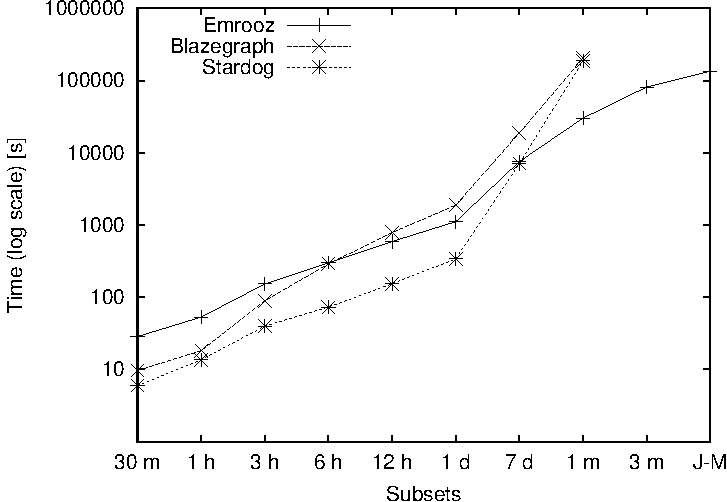
\includegraphics[scale=0.6]{load-performance-plot.pdf}
	\caption{Load performance for the subsets and Emrooz compared to Stardog and Blazegraph. Stardog and Blazegraph evaluations did not terminate on time for this paper.}
	\label{fig:load-performance-plot}
\end{figure}

% DISCUSSION
Compared to Stardog and Blazegraph, and comparable triple stores, Emrooz has some constraints. Most obviously, Emrooz cannot manage arbitrary RDF data. Furthermore, Apache Cassandra has no means to perform standard reasoning tasks on SSN observations. Off-the-shelf reasoning can only be performed by Sesame, on the knowledge store and in post-processing query result sets returned by Apache Cassandra. Some level of reasoning pushed down to the Apache Cassandra data store can be implemented by Emrooz using the Sesame knowledge store and query rewriting \cite{kontchakov14rewriting}.

\begin{figure}
	\centering
	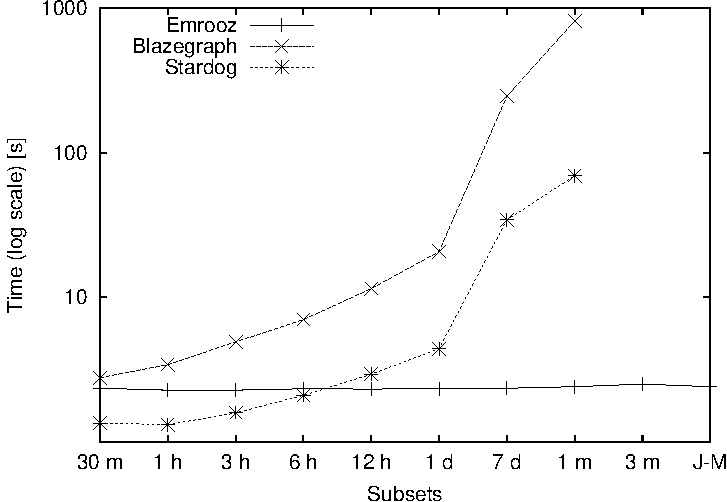
\includegraphics[scale=0.6]{query-performance-plot.pdf}
	\caption{Query performance for the subsets and Emrooz compared to Stardog and Blazegraph. Stardog and Blazegraph evaluations did not terminate on time for this paper.}
	\label{fig:query-performance-plot}
\end{figure}

Emrooz is currently capable of evaluating SPARQL queries with a basic graph pattern for SSN observations, whereby the observation result time must be constrained by a time interval $[\dot{t}_1,\dot{t}_2[$ specified as \texttt{FILTER}. The related sensor, property, and feature may be bound or unbound. SPARQL features such as aggregates and solution modifiers such as \texttt{ORDER BY} can be specified over $[\dot{t}_1,\dot{t}_2[$.

Sesame post-processing adds overhead which can be avoided if applications do not require SPARQL. SPARQL adds flexibility, e.g. it enables selecting variables, ordering or filtering results. However, in some applications this flexibility may not be required and does thus not justify the overhead. For instance, a data portal may simply want to return the set of RDF statements matching the user query $q_{so} \leftarrow (\dot{s},\dot{p},\dot{f},\dot{t}_1,\dot{t}_2)$ and leave further processing to the user.

The data in our case study arguably fall into the category of ``particularly hard cases'' for triple stores. Assuming equally sized datasets, SSN observation query evaluation on data collected from sensor networks with more sensors, properties, and features but sampling at lower frequency are less expensive for triple stores. This is because the tuple $(\dot{s},\dot{p},\dot{f})$, as well as its elements, are more selective. The intermediate result sets are smaller and basic graph pattern joins less expensive. Furthermore, more diverse selectivity estimates for triple patterns could give query optimizers more room to find better query plans.

\section{Related and Future Work}
\label{s:related-and-future-work}
A number of authors have developed RDF data management systems that build on NoSQL stores such as Apache Cassandra. Cudr{\'e}-Mauroux et al. \cite{harith13nosql} provide a comparative evaluation for the load and query performance of several systems that implement an RDF data management layer on top of a NoSQL system. Of particular interest here is CumulusRDF \cite{ladwig11cumulusrdf}, as it also builds on Apache Cassandra and Sesame. However, these systems aim at being RDF databases and thus implement indexes specialized for answering arbitrary SPARQL queries on RDF. In contrast, Emrooz is designed for the management of SSN observations represented in RDF and for the evaluation of SSN observation queries formulated in SPARQL. Emrooz is thus designed to be a scalable time series database for sensor observations represented in RDF according to the vocabulary defined by the SSN ontology.

Authors who developed systems for (historical or streamed) sensor data management have recognized that persisting large volumes of sensor data in an RDF database is hardly viable. Presenting a platform designed to connect (semantic) sensor data with data in the `Linked Data Cloud', Le-Phuoc et al. \cite{phuoc11linked} resort to a relational database management system for historical sensor data management. Describing a data warehouse for water resource management, Abecker et al. \cite{abecker14sensor} also propose a hybrid approach in which time series sensor data is managed by a relational database system (PostGIS) whereas information objects with more complex relationships are managed by an RDF database. The authors note that ``a complete `semantification' [...] of all data [...] seemed not feasible and promising to us, especially regarding the measurement data.''

NoSQL systems have been utilized to manage SSN observations, specifically. Wang et al. \cite{wang14hdsw} present a Hadoop-based system designed to manage SSN observations. The authors describe how their system stores SSN observations to HBase which, however, features an index structure that is typical for RDF statements, akin to the systems surveyed by Cudr{\'e}-Mauroux et al. \cite{harith13nosql}. Wang et al. evaluate the performance of various queries. However, to our understanding the queries are not for SSN observations but rather for single triple patterns, e.g. a pattern with bound subject and unbound predicate and object. As such, both the indexing approach and the query performance evaluation are different from those presented in this paper for Emrooz.

There are several potentially interesting directions for future work. First, we plan to extend the implementation so that it supports the management of \emph{dataset} observations represented following the RDF Data Cube (QB) Vocabulary \cite{cyganiak13qb}. With this extension, Emrooz could thus manage not only raw sensor data but also processed sensor data. For instance, \ce{CO2} flux sensor data are used to compute Net Ecosystem Exchange (NEE). NEE data are a result of sensor data processing and form a dataset; hence the different vocabulary. Combining the SSN ontology and the QB vocabulary in systems has been demonstrated in the literature, e.g. \cite{lefort12qb,stocker13ems}.

Second, Emrooz can be equipped with further features. Command line tools could simplify user interaction with Emrooz. A RESTful service could expose (load) and query functionality for client-server interaction over HTTP. A browser-based client could support the visualization of time series. R\footnote{http://www.r-project.org/} and Matlab\footnote{www.mathworks.com/products/matlab/} libraries could enable users to query and persist data from statistical computing environments. Data managed by Emrooz could then be loaded into R data frames. Results of computations in R could be persisted in Emrooz. Finally, Emrooz could be enhanced with more flexibility in SPARQL query formulation, e.g. filter for a set of properties, as well as reasoning at query time. These enhancements could be supported by extending the existing query rewriting mechanism. A detailed analysis of the SPARQL expressivity covered in Emrooz may also be of interest.

Third, it is interesting to compare Emrooz performance with triple stores that build on SQL and NoSQL databases, such as SDB\footnote{https://jena.apache.org/documentation/sdb/} and CumulusRDF \cite{ladwig11cumulusrdf}, respectively, as well as with non-triple stores, including SQL or OGC standards compliant databases, such as PostgreSQL\footnote{http://www.postgresql.org/} and 52North,\footnote{http://52north.org/} respectively.

\section{Conclusion}
\label{s:conclusion}
We have presented a scalable database for sensor observations represented in RDF capable of evaluating queries for sensor observations formulated in SPARQL. We briefly discussed how the database builds on Apache Cassandra and Sesame for its implementations of a data store and a knowledge store, respectively, and how the two stores interact. As we demonstrated for two state-of-the-art triple stores, sensor observation query evaluation becomes quickly prohibitive as store size grows to tens of millions sensor observations. To serve client applications with sensor observations in RDF is attractive for several reasons, including data linked to metadata and formal descriptions of vocabulary semantics. However, for practical viability the underlying sensor observations management system needs to be designed for time series query evaluation.

\section*{Acknowledgements}
\label{s:acknowledgements}
This research is funded by the Academy of Germany project ``ROTAR: High-quality Measurement Infrastructure'' (Grant number 5489654).

%% The Appendices part is started with the command \appendix;
%% appendix sections are then done as normal sections
%% \appendix

%% \section{}
%% \label{}

%% If you have bibdatabase file and want bibtex to generate the
%% bibitems, please use
%%
\bibliographystyle{elsarticle-harv} 
\bibliography{<your bibdatabase>}

%% else use the following coding to input the bibitems directly in the
%% TeX file.

% \begin{thebibliography}{00}

%% \bibitem[Author(year)]{label}
%% Text of bibliographic item

% \bibitem[ ()]{}

% \end{thebibliography}
\end{document}

\endinput
%%
%% End of file `elsarticle-template-harv.tex'.
